\documentclass[tikz,border=8pt]{standalone}
\usepackage[T1]{fontenc}
\usepackage{times}
\usetikzlibrary{arrows.meta,positioning}
\begin{document}
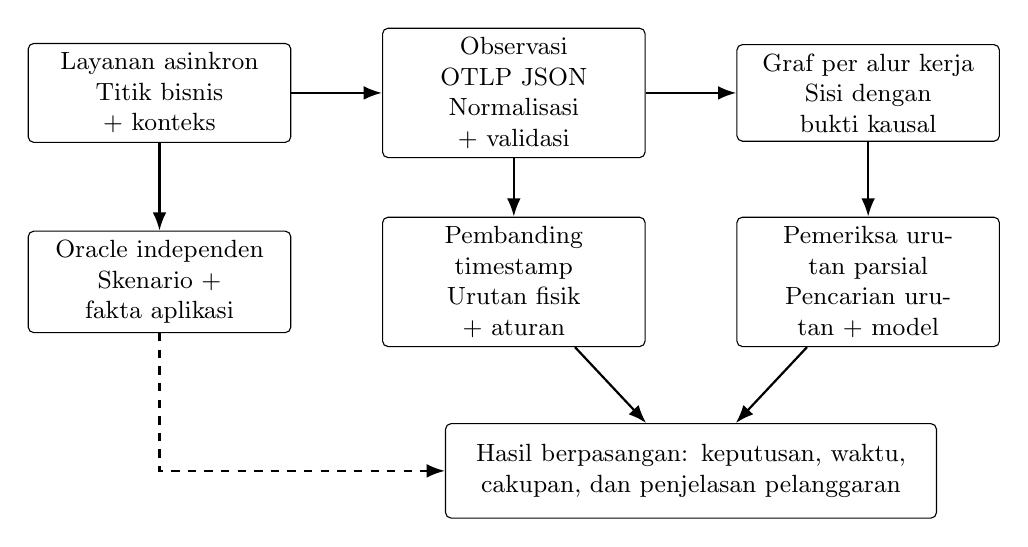
\begin{tikzpicture}[box/.style={draw,rounded corners=2pt,align=center,
  text width=3.1cm,minimum height=1.2cm,font=\small},
  arrow/.style={-{Latex},thick}]
  \node[box] (app) at (0,0) {Layanan asinkron\\Titik bisnis + konteks};
  \node[box] (obs) at (4.5,0) {Observasi OTLP JSON\\Normalisasi + validasi};
  \node[box] (graph) at (9,0) {Graf per alur kerja\\Sisi dengan bukti kausal};
  \node[box] (oracle) at (0,-2.4) {Oracle independen\\Skenario + fakta aplikasi};
  \node[box] (baseline) at (4.5,-2.4) {Pembanding timestamp\\Urutan fisik + aturan};
  \node[box] (verifier) at (9,-2.4) {Pemeriksa urutan parsial\\Pencarian urutan + model};
  \node[box,text width=6cm] (report) at (6.75,-4.8)
    {Hasil berpasangan: keputusan, waktu,\\cakupan, dan penjelasan pelanggaran};
  \draw[arrow] (app) -- (obs);
  \draw[arrow] (obs) -- (graph);
  \draw[arrow] (obs) -- (baseline);
  \draw[arrow] (graph) -- (verifier);
  \draw[arrow] (app) -- (oracle);
  \draw[arrow] (baseline) -- (report);
  \draw[arrow] (verifier) -- (report);
  \draw[arrow,dashed] (oracle.south) |- (report.west);
\end{tikzpicture}
\end{document}
